\section{Result}
\section{Simulation Studies}
The simulations are based on the real NGS and MRI data of 806 ADNI participants with both profiles. Each iteration run choose a pair of genomic and cortical testing units. The genomic testing unit is a gene with 5kp upstream and downstream flanking window. As for the cortex, a testing unit is a region of 512 vertices randomly picked from the entire cortical surface, which is is roughly an oval of 2.8mm in diameter. The genomic effect and vertex effect are simulated by assigning values drawn from standard normal distribution to a certain percentage of the variants randomly selected from a testing unit (e.g. polymophisms in a gene or vertices in an oval cortical region). The purely genomic and vertex based response are then generated as the product of the testing unit with the simulated effect. An additive and an interactive response are also created by adding up the two basic responses, with and without an additional element-wise product of the two. Lastly, we assign some noise to the generated responses. For now we will focuse on continous respones, the simulation study for dichotomous responses will be covered later.

\noindent\textbf{Robustness of the Joint U} \\
The first set of study aims to test the robustness of the joint U statistics $U_J$ under very likely circumstances of model mis-specification. The power performance of the joint U is compared with the two simpler statistics without either genomic or vertex kernel function. The performance under 8 sample size setting and the 4 scenarios of effect composition is shown in Figure \ref{fig:PWR_CNT_KNL}.
\begin{figure}[!htbp]
\label{fig:PWR_CNT_KNL}
\centering
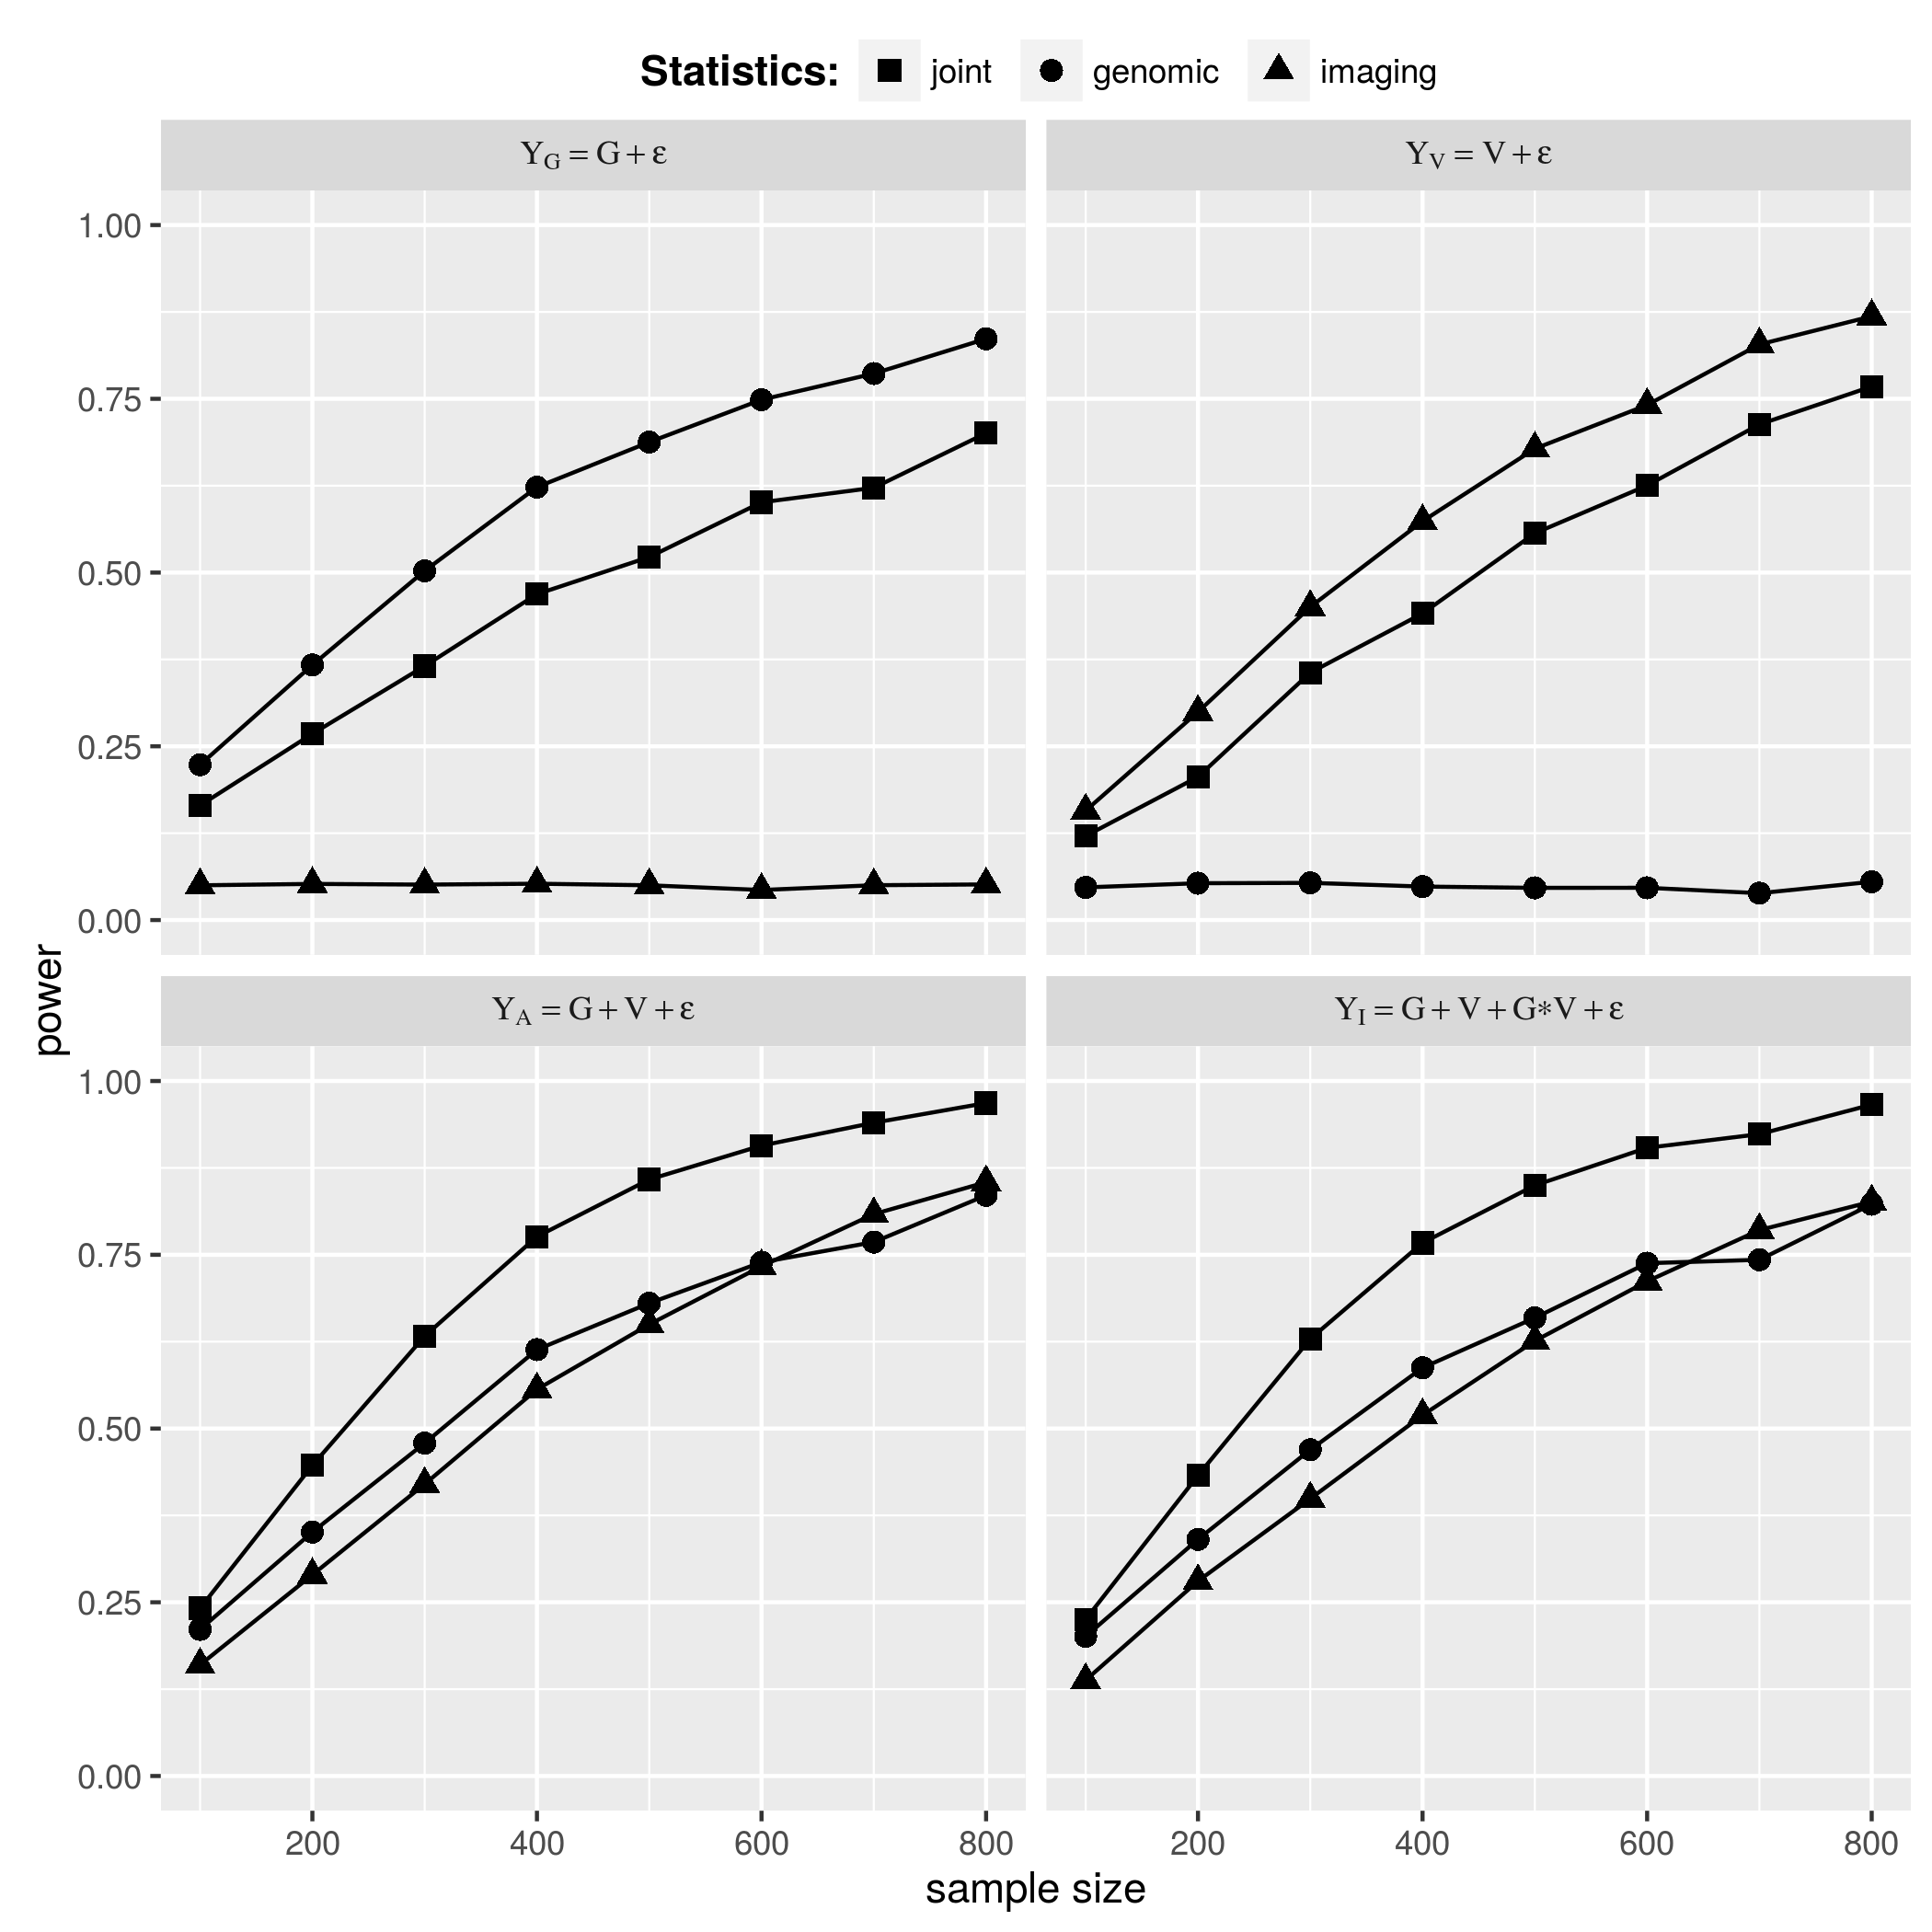
\includegraphics[width=300px]{img/PWR_CNT_KNL.png}
\caption{Joint U v.s. Parsimonious U statistics}
\end{figure}
The top row of Figure \ref{fig:PWR_CNT_KNL} shows that, the two parsimonious statistics $U_G$ and $U_V$ performed the best when the underlying effects were indeed purely genomic and vertex backed, respectively, but they are completely powerless when the actual effect compostion do not concure with their choice of U-kernel functions. In constrast, the joint statistic $U_J$ performed fairly well under both circumstances, close to the optimal power displayed by correlty specified parsimonious models. The bottom row of Figure \ref{fig:PWR_CNT_KNL} shows joint U statistic $U_J$ outperformed both $U_G$ and $U_V$ when the effect is additve, either with (Figure \ref{fig:PWR_CNT_KNL} down left) or without (Figure \ref{fig:PWR_CNT_KNL} down right) an additional interaction term.

\noindent \textbf{Grouping and Aggregation on Vertices} \\
We known vertices in a cortax profile do not have ``low MAF'' issue that rare genomic variants have, but the grouping and aggregation strategy used by analysis of NGS data may still benefit analysis involving cortial surfaces. The second study aims to see weather an aggregated cortical testing unit achieve higher power than the per-vertex based VWA followed by FDR (false discovery rate) correction. Comparison of the two strategy is done under the same 8 sample size and 4 effect compositions, but without the $U_G$ statistics since it does not involves cortex profile. The result is shown in Figure \ref{fig:PWR_CNT_VWA}.
\begin{figure}[!htbp]
\label{fig:PWR_CNT_VWA}
\centering
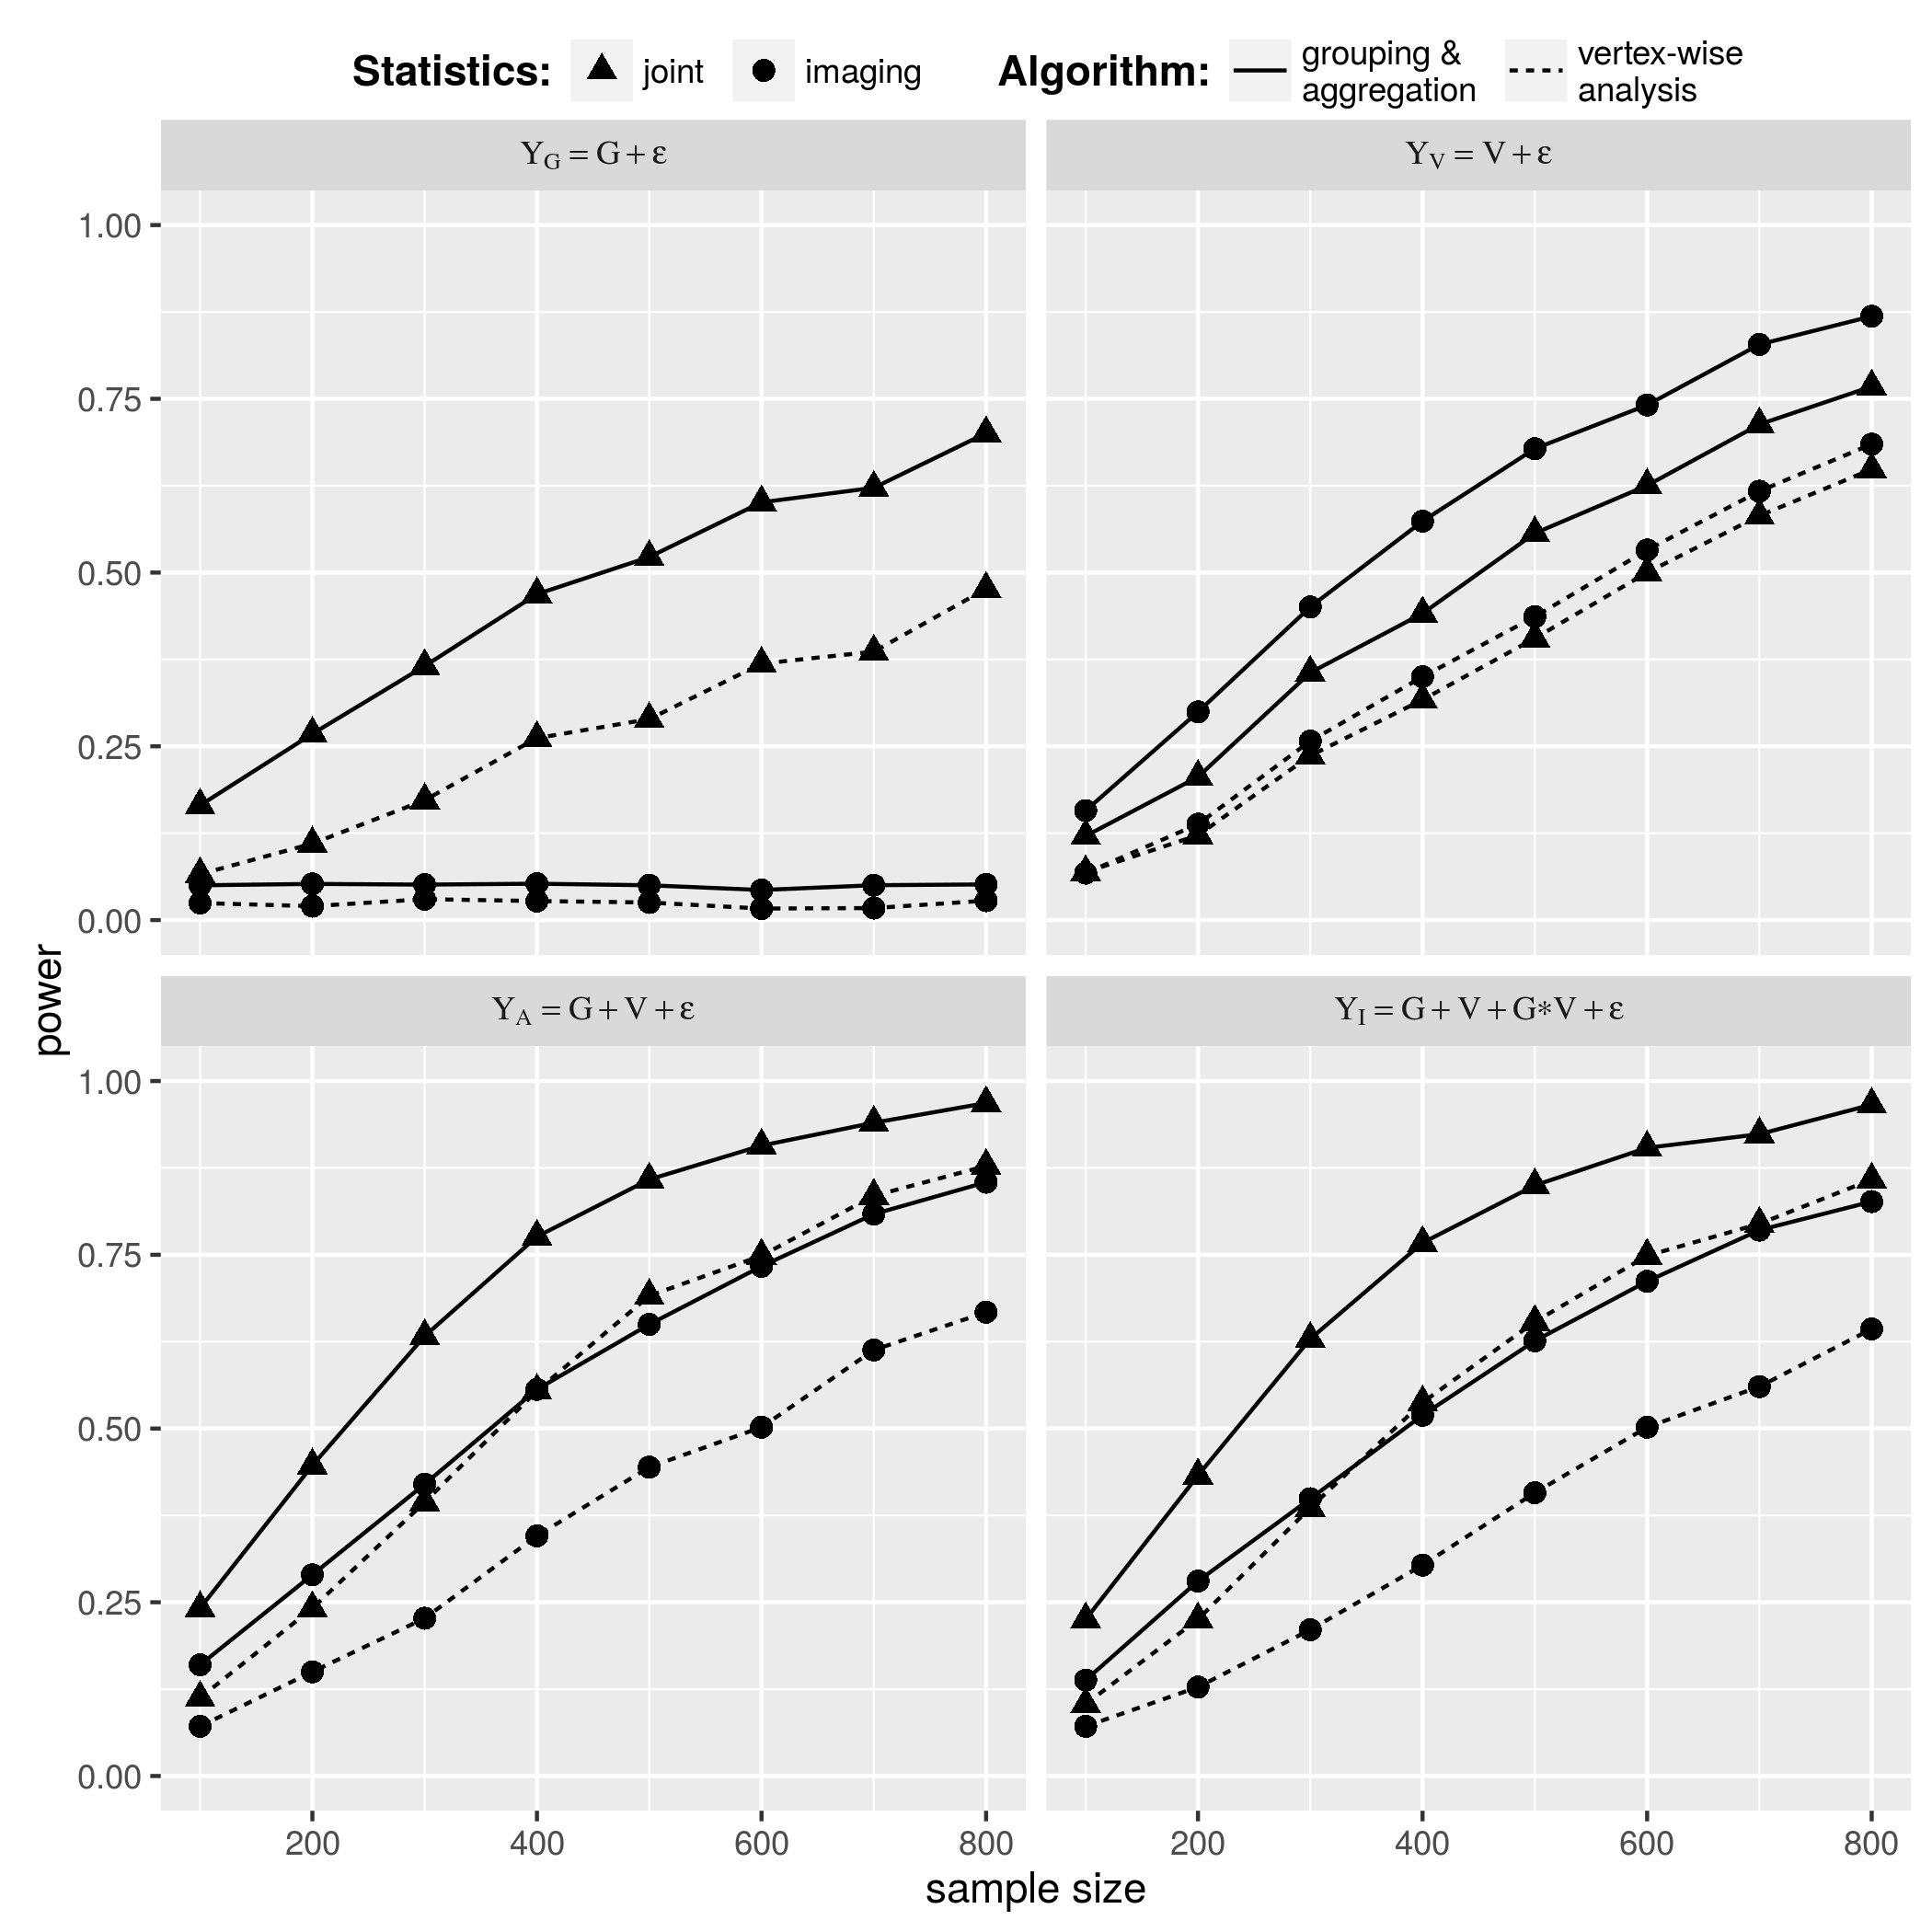
\includegraphics[width=300px]{img/PWR_CNT_VWA.png}
\caption{Vertex Grouping \& Aggregation v.s. Vertex-wise Analysis}
\end{figure}
Under all simulation settings, the aggregated testing unit (solid lines) overpowers the per-vertex based VWA (dashed lines). This gap is only slightly closed when the sample size grows large. Another interesting speculation is when the U kernel functions is totally mis-specified, the type I error rate of VWA is lower then the 0.05 threshold while the aggregated test isn't (Figure \ref{fig:PWR_CNT_VWA}, top left panel). The multiple testing correction is done by false discover rate (FDR) adjustment, which says that the adjusted p-value will be conservative if the tests were not independent. Therefore, a conservative type I error rate refects the fact that closely located vertices are correlated as they were sampled from tightly connected brain tissue. As a result, grouping and signal aggregation is also recommended for cortex profile.

Another issue worth mentioning is the performance issue. The VWA takes drastically more time than the grouping and aggregation approach, because it has to perfrom $|V|$ tests in order to derive one final $U_V$ or $U_J$ statistic instead of just once. For now, the simulation study fixes $|V|$ to 512, under the largest sample size, 800, a single run of the proposed method using 1 cpu core takes only a few seconds, but the VWA approach paralleled on 4 cpu cores requires nearly 4 hours.

\noindent \textbf{Abstract High Order Features from Cortex Vertices}
The third set of study tests whether the high order features abstracted from the raw cortex profile provides higher statistical power than the raw profile itself. Again the comparisons is done under all settings except those involving $U_G$ that doesn't rely on vertices in the cortex. The result is shown in Figure \ref{fig:PWR_CNT_SAE}.
\begin{figure}[!htbp]
\label{fig:PWR_CNT_SAE}
\centering
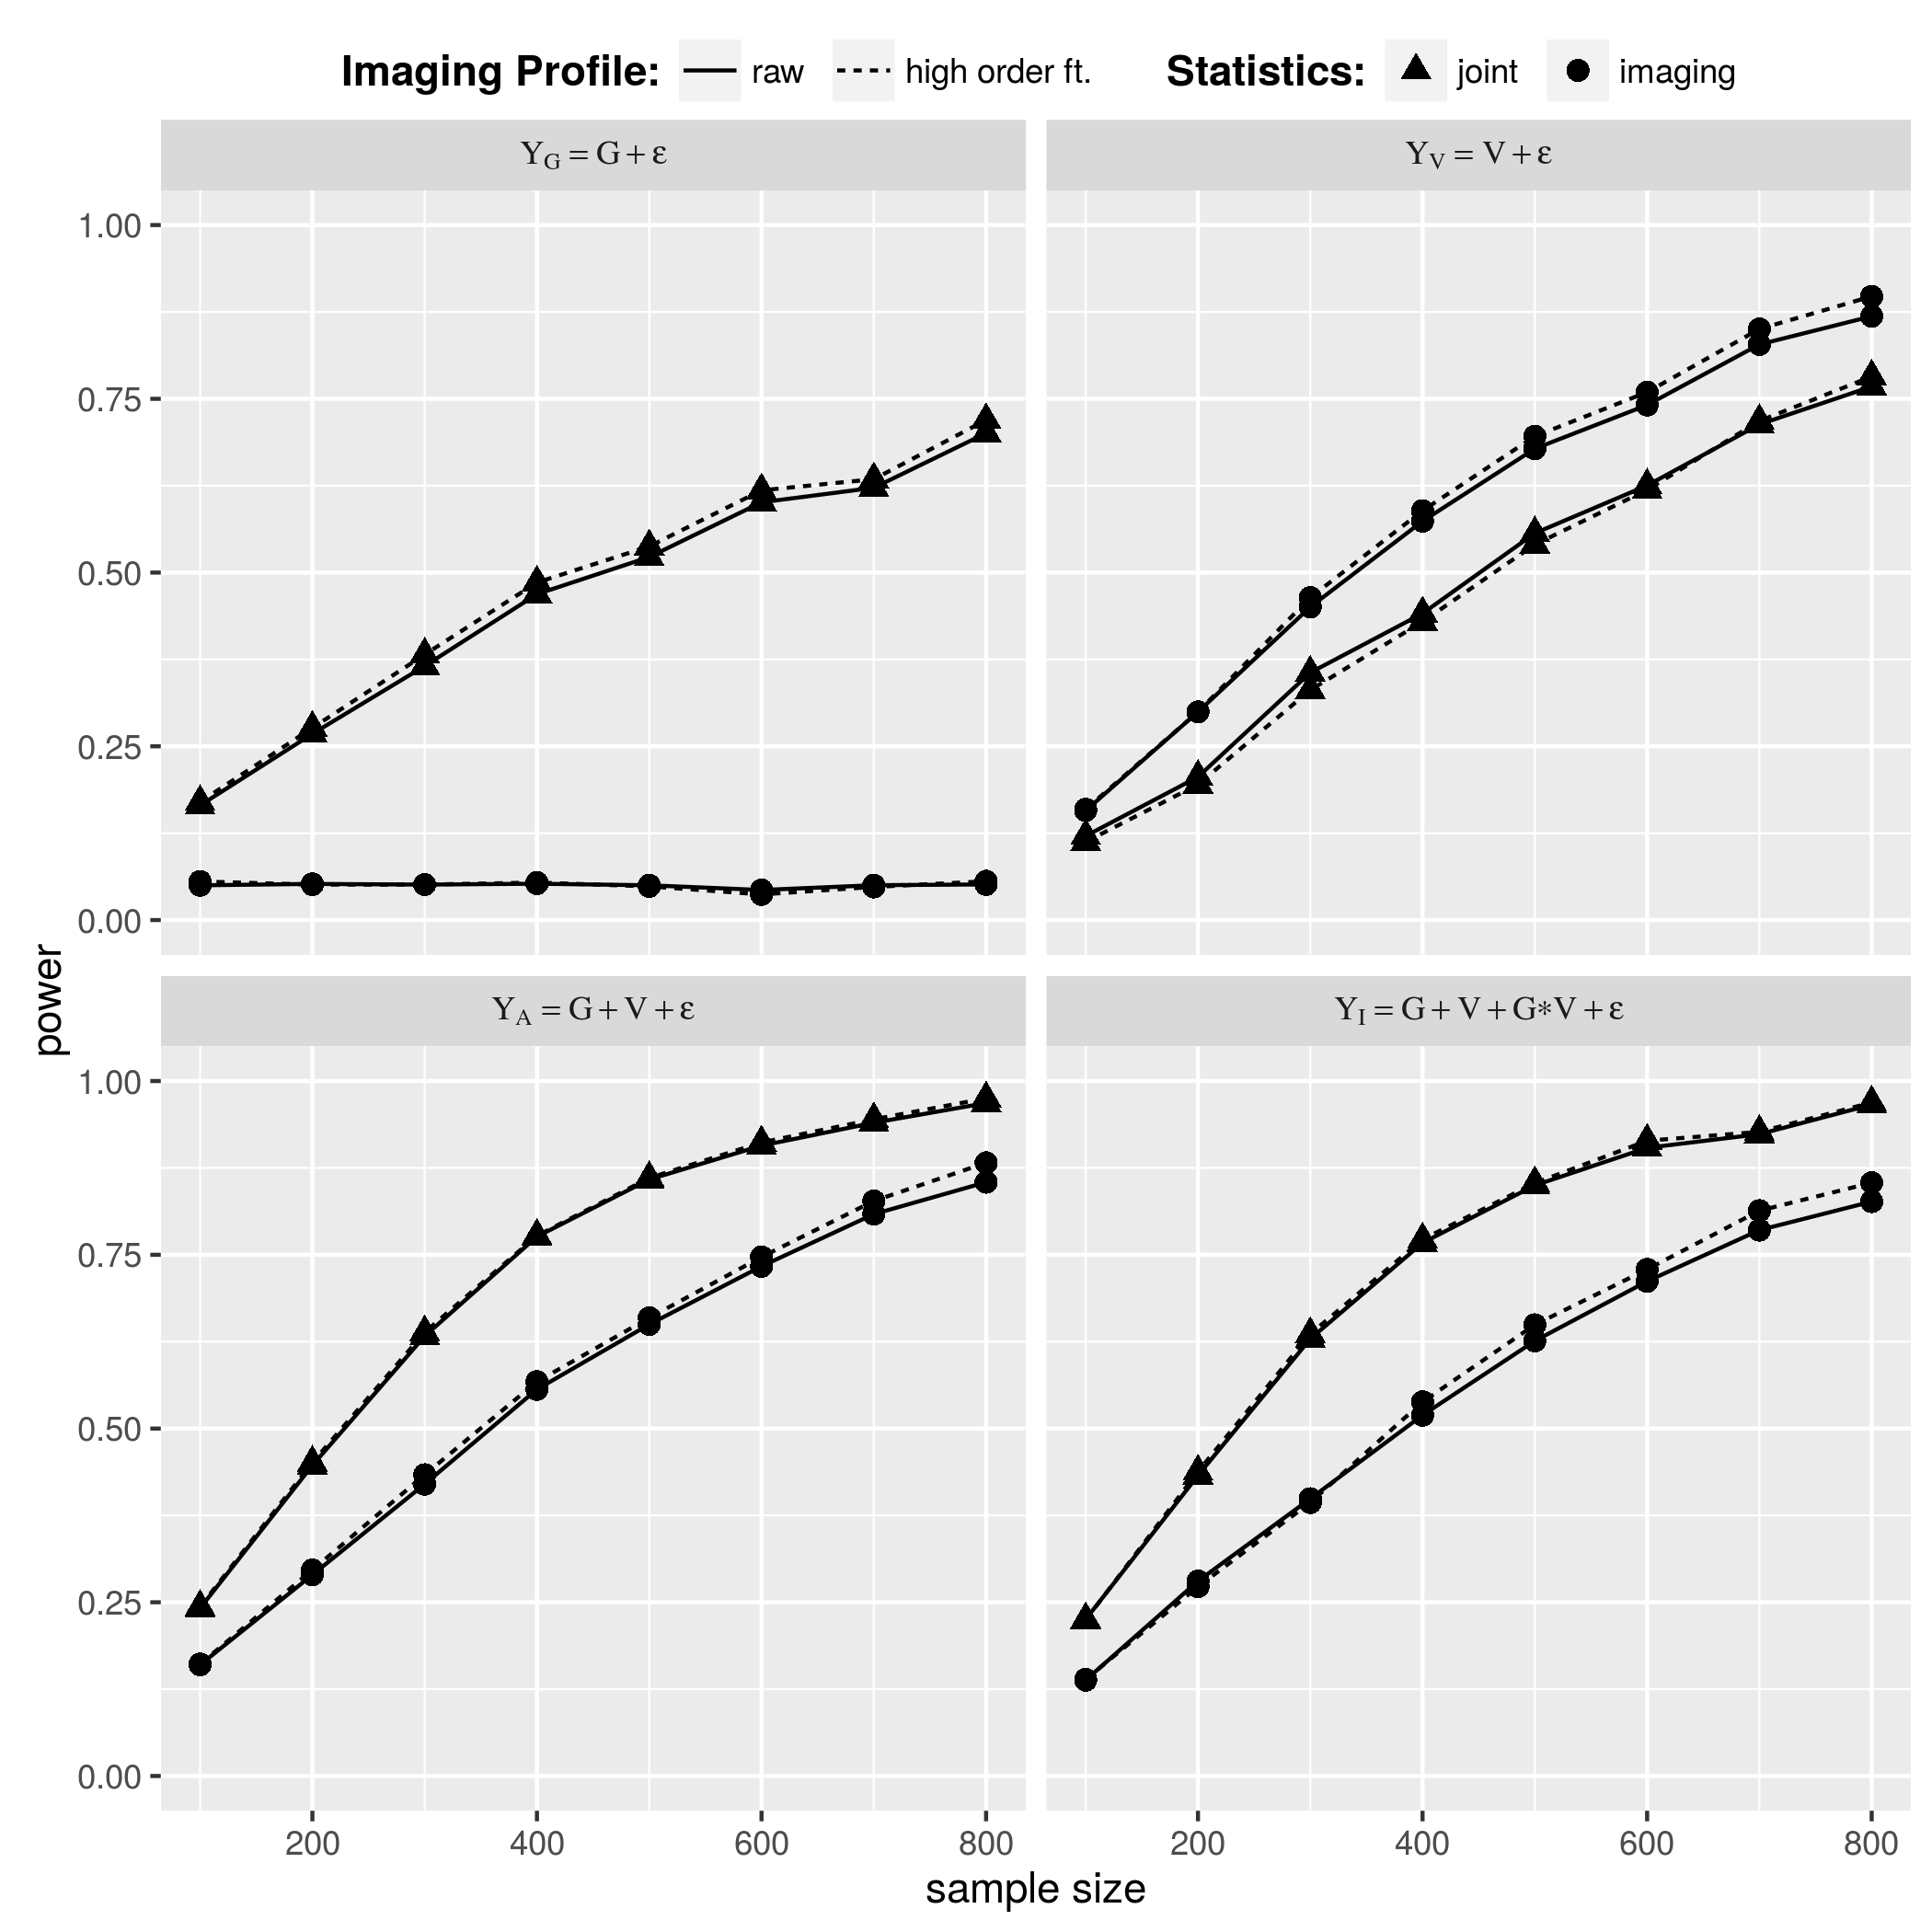
\includegraphics[width=300px]{img/PWR_CNT_SAE.png}
\caption{High Order Features v.s. Orignal Vertices}
\end{figure}
In most scenarios, the abstracted features (Figure \ref{fig:PWR_CNT_SAE}, dashed lines) offers more power then the orignal vertices (Figure \ref{fig:PWR_CNT_SAE}, solid lines), and the edge is growing with the sample size become larger. The only exception happened when the sample size is lower then 600, the effect is purely vertex based, and the partially mis-specified joint U statistic is used for the test (Figure \ref{fig:PWR_CNT_SAE}, top right). Since the rejection of null hypothesis counts as type I error when the kernel functions are complete mis-sepcified, the top left panel in \ref{fig:PWR_CNT_SAE} shows that, the use of abstracted features doesn't deviate the type I error rate from the 0.05 threshold.

\textbf{Simulation study of Binary phenotypes}
The dichotomous responses is simulated by pluging the continuous responses into inverse logit function to get an array of probabilities, then draw the binary case/control status from these probabilities. The power performace shares very similar patterns under every scenario, albeit poorer then its continuous counterpart. The results is shown in Figure \ref{fig:PWR_BIN_KNL}, \ref{fig:PWR_BIN_VWA} and \ref{fig:PWR_BIN_SAE}.

In general, the simulation studies have so far demenstrated the robustness and versitility of the proposed method when faced with uncertain effect composition and a variety of phenotype distributions. Also shown is the helpfulness of groupping and aggregation strategy used by many rare genomic variant studies over other types of high dimenstional whose variants are not ``rare'' but potentlly correlated. The power boost offered by the stacked autoencoders is not dramatic, but is increasingly more positive when the sample size grows.

\subsection{Real Data Analysis}
The baseline data of 327 out of 806 participants who has definite diagnosis status entered the analysis. The genomic testing units are still defined by gene. The image testing units are now 68 cortical anatomy regions except bankssts in the right hemispheres. These 67 sets of vertices are sent to 67 cooresponding stacked autoencoders trained with all 806 profiles, the resulting 67 sets of high order features are then combined with the genes to perform the joint U statistic test. The total number of joint U statistics is $40,039 \times 67 = 2,680,894$, that is, the number of genes times the number of cortical regions. Among the 327 choosen subjects, 47 of them are diagnosed with either Alzheimer's disease (AD) or dementia, while the rest 280 subjests are healthy controls (CN). The case/control outcomes were first regressed on 7 known risk factors of AD, namely age, gender, race, ethnicity, years of education, marriage status, ever smoking, and APOE $\epsilon$4 haplotype. The regression residuals were then taken as the actual phenotype. For each tuple of gene and cortical region, we also derive $U_G$ and $U_V$ to test the two simplified null hypothesis. Thus, the results came in triplets of p-values $P_G$, $P_V$ and $P_U$, corresponding to the three U statistics $U_G$, $U_V$, and $U_J$. After negative log transformation, the triplets are show in Figure \ref{fig:RDA_PVL} horizontally, order by the transform $U_J$.
\begin{figure}[!htbp]
\centering
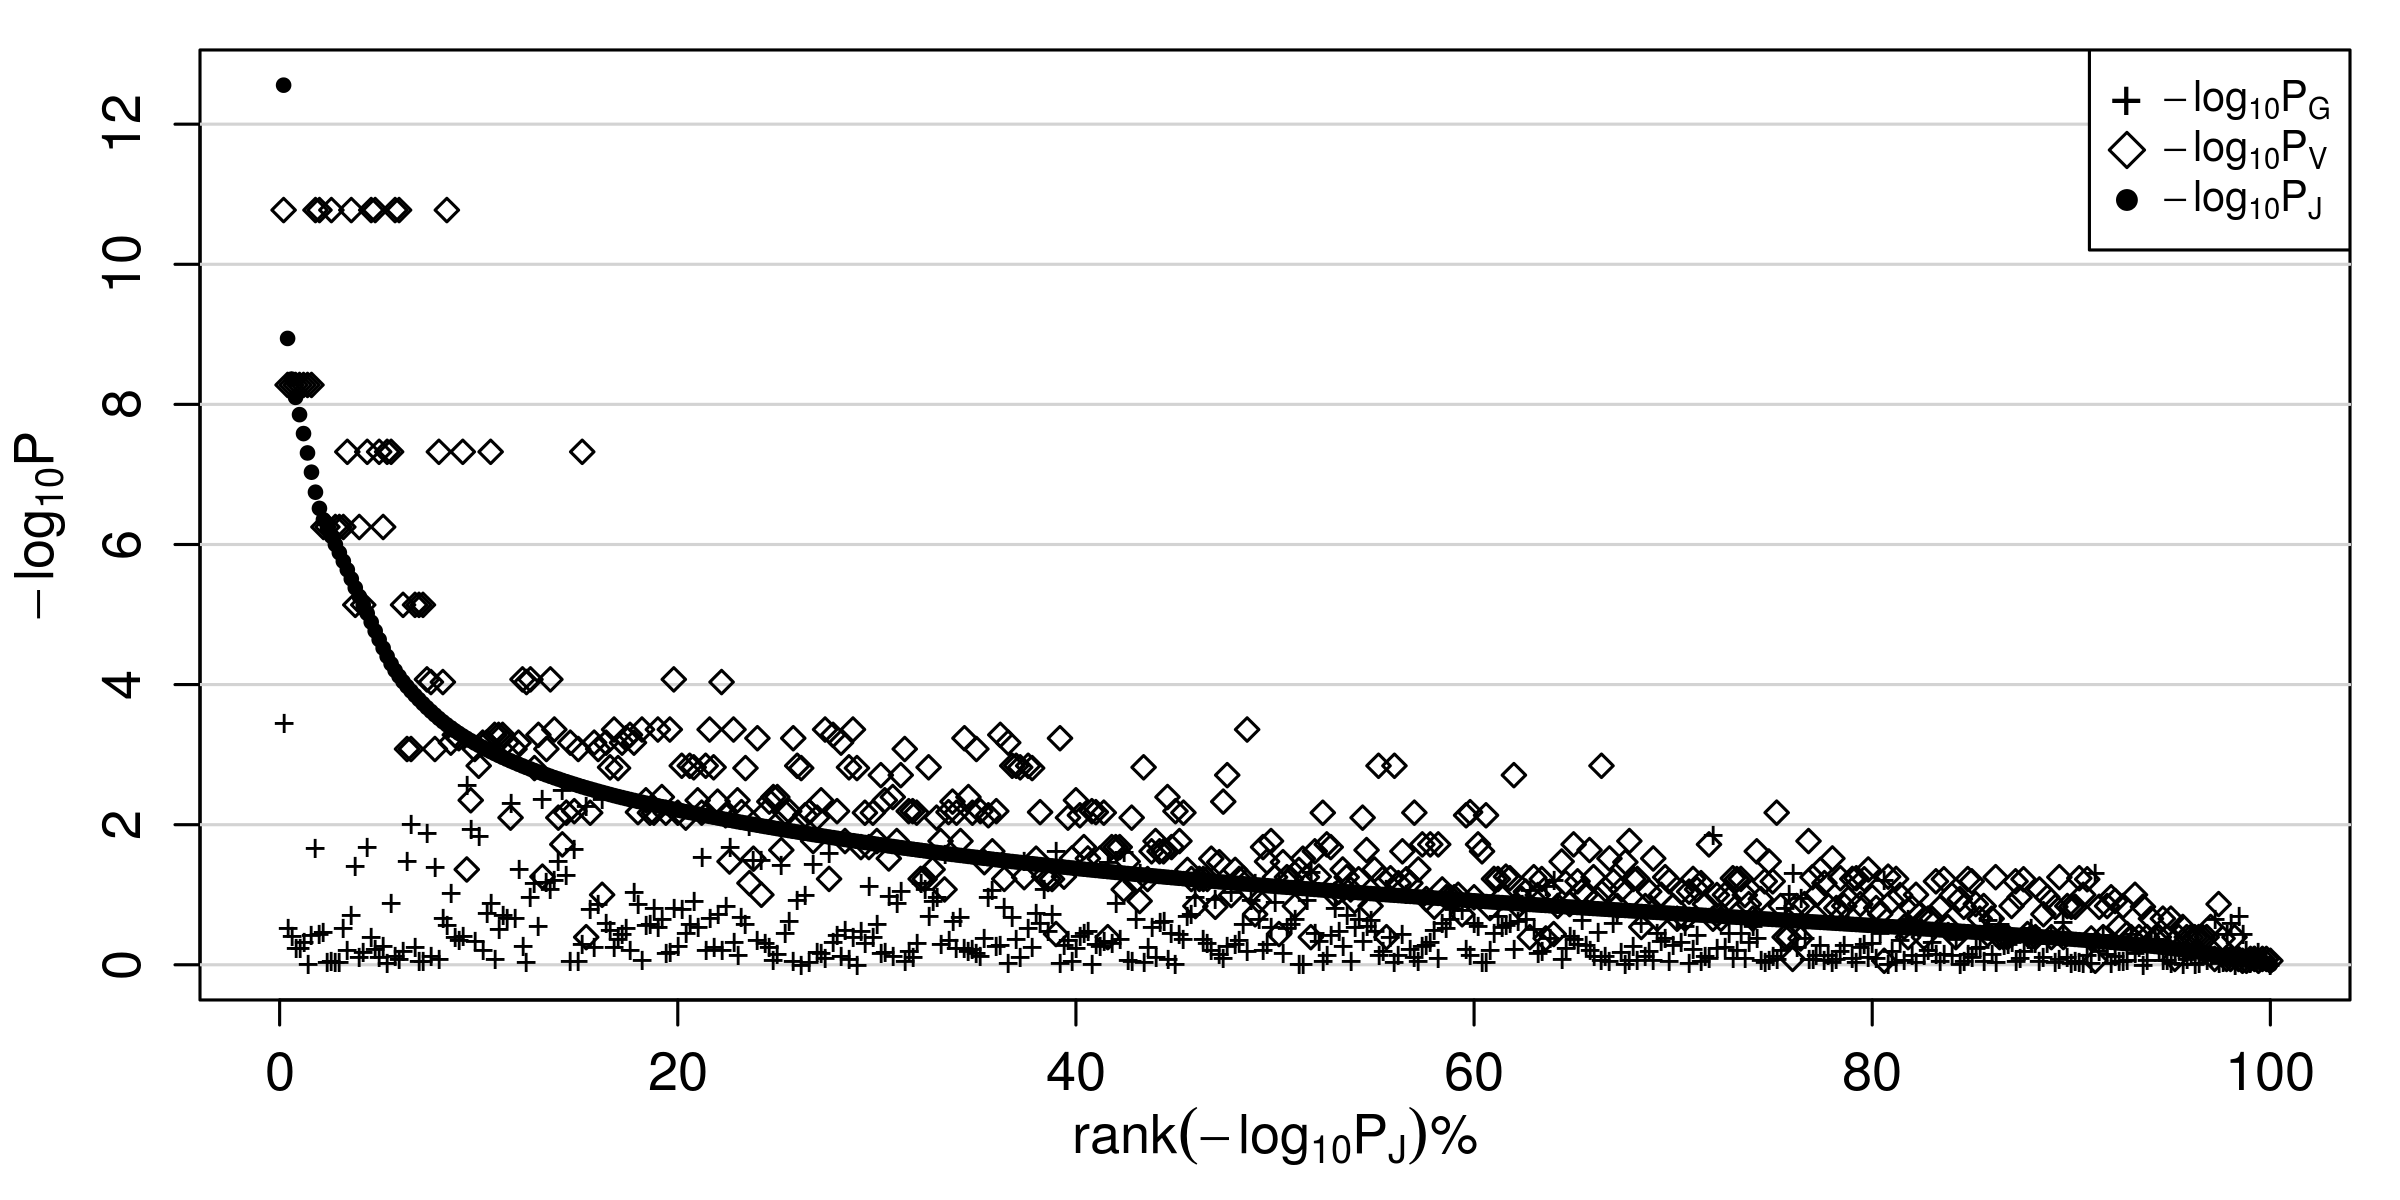
\includegraphics[width=\textwidth]{img/RDA_PVL.png}
\caption{p-values of real data analysis}
\label{fig:RDA_PVL}
\end{figure}
In general, the significance of the purely vertex based $U_G$ (Figure \ref{fig:RDA_PVL} diamonds) is above the purely genomic based $U_G$ (Figure \ref{fig:RDA_PVL} crosses), reflecting the fact that genomic effect is weak while the cortex profile is a very indicator of the diseases in brain, and the joint similarity U statistic $U_J$ (Figure \ref{fig:RDA_PVL} dots) lies between the two, leaning closer to the cortical vertex based $U_V$. To be noted is how $U_J$ ``borrow'' information from the cortex profile to enhance the statistical significance of the purely genomic based $U_G$, which by itself never reaches significance at the threshold of $0.05$ after the FDR adjustment of $40,039$ tests. When $U_G$ is also moderately significant, the corresponding joint statistic $U_J$ could be more significant than both $U_G$ and $U_V$, reaching the 0.05 threshold even after FDR adjustment over $2,680,894$ tests, which is shown by the dots in the most top left corner of Figure \ref{fig:RDA_PVL}, and reflected by the 20 top significant triplets listed in Table \ref{tab:RDA_T20}.
\begin{table}[!htbp]
\centering
% latex table generated in R 3.3.1 by xtable 1.8-0 package
% Fri Dec 23 17:55:43 2016
\begin{tabular}{llcclll}
  \hline
  GENE & CORTEX & $|V|$ & $|G|$ & $\qquad P_G$ & \qquad $P_V$ & \qquad $P_J$ \\ 
  \hline
  IGLV1-44 & l.superiortemporal & 7271 &  174 & $3.51 \times {10^{-04}}$ & $1.68 \times {10^{-11}}{_+^*}$ & $2.77 \times {10^{-13}}{_+^*}$ \\ 
  NBEAP2 & l.superiortemporal & 7271 &  238 & $1.19 \times {10^{-04}}$ & $1.68 \times {10^{-11}}{_+^*}$ & $4.74 \times {10^{-13}}{_+^*}$ \\ 
  RPL21P89 & l.superiortemporal & 7271 &   90 & $6.36 \times {10^{-04}}$ & $1.68 \times {10^{-11}}{_+^*}$ & $5.14 \times {10^{-13}}{_+^*}$ \\ 
  LOC102724504 & l.superiortemporal & 7271 &   59 & $1.41 \times {10^{-03}}$ & $1.68 \times {10^{-11}}{_+^*}$ & $5.56 \times {10^{-13}}{_+^*}$ \\ 
  CNTNAP3P8 & l.superiortemporal & 7271 &   40 & $1.08 \times {10^{-03}}$ & $1.68 \times {10^{-11}}{_+^*}$ & $6.17 \times {10^{-13}}{_+^*}$ \\ 
  CDH4 & l.superiortemporal & 7271 & 9464 & $4.64 \times {10^{-03}}$ & $1.68 \times {10^{-11}}{_+^*}$ & $6.96 \times {10^{-13}}{_+^*}$ \\ 
  HNRNPA1P19 & l.superiortemporal & 7271 &   17 & $8.88 \times {10^{-04}}$ & $1.68 \times {10^{-11}}{_+^*}$ & $7.80 \times {10^{-13}}{_+^*}$ \\ 
  FAM72C & l.superiortemporal & 7271 &  174 & $9.28 \times {10^{-06}}$ & $1.68 \times {10^{-11}}{_+^*}$ & $7.82 \times {10^{-13}}{_+^*}$ \\ 
  RP11-638L3.1 & l.superiortemporal & 7271 & 4067 & $1.41 \times {10^{-1}}$ & $1.68 \times {10^{-11}}{_+^*}$ & $9.49 \times {10^{-13}}{_+^*}$ \\ 
  CPXM1 & l.superiortemporal & 7271 &  208 & $8.78 \times {10^{-4}}$ & $1.68 \times {10^{-11}}{_+^*}$ & $1.08 \times {10^{-12}}{_+^*}$ \\ 
  LOC101929612 & l.superiortemporal & 7271 &  256 & $1.44 \times {10^{-2}}$ & $1.68 \times {10^{-11}}{_+^*}$ & $1.15 \times {10^{-12}}{_+^*}$ \\ 
  LOC100996517 & l.superiortemporal & 7271 &   34 & $6.77 \times {10^{-4}}$ & $1.68 \times {10^{-11}}{_+^*}$ & $1.20 \times {10^{-12}}{_+^*}$ \\ 
  IGLV5-45 & l.superiortemporal & 7271 &  179 & $3.44 \times {10^{-4}}$ & $1.68 \times {10^{-11}}{_+^*}$ & $1.23 \times {10^{-12}}{_+^*}$ \\ 
  MIS18BP1 & l.superiortemporal & 7271 &  553 & $4.95 \times {10^{-3}}$ & $1.68 \times {10^{-11}}{_+^*}$ & $1.35 \times {10^{-12}}{_+^*}$ \\ 
  CDR2 & l.superiortemporal & 7271 &  260 & $1.82 \times {10^{-4}}$ & $1.68 \times {10^{-11}}{_+^*}$ & $1.39 \times {10^{-12}}{_+^*}$ \\ 
  RPL41P2 & l.superiortemporal & 7271 &   87 & $6.04 \times {10^{-3}}$ & $1.68 \times {10^{-11}}{_+^*}$ & $1.59 \times {10^{-12}}{_+^*}$ \\ 
  LOC101927737 & l.superiortemporal & 7271 &  157 & $7.20 \times {10^{-3}}$ & $1.68 \times {10^{-11}}{_+^*}$ & $1.60 \times {10^{-12}}{_+^*}$ \\ 
  IGLV1-47 & l.superiortemporal & 7271 &  138 & $1.44 \times {10^{-2}}$ & $1.68 \times {10^{-11}}{_+^*}$ & $1.60 \times {10^{-12}}{_+^*}$ \\ 
  IGLV7-46 & l.superiortemporal & 7271 &  130 & $9.15 \times {10^{-4}}$ & $1.68 \times {10^{-11}}{_+^*}$ & $1.69 \times {10^{-12}}{_+^*}$ \\ 
  ZDHHC15 & l.superiortemporal & 7271 &   80 & $1.56 \times {10^{-3}}$ & $1.68 \times {10^{-11}}{_+^*}$ & $1.73 \times {10^{-12}}{_+^*}$ \\ 
  \hline
  \multicolumn{7}{l}{\texttt{*: below 0.05 after Bonferroni correction}} \\ 

  \multicolumn{7}{l}{\texttt{+: below 0.01 after FDR correction}}        \\ \hline
\end{tabular}

\caption{top 20 most significant joint test - overall}
\label{tab:RDA_T20}
\end{table}
From Table \ref{tab:RDA_T20} we see the top 20 most significant test all involves the left superiortemporal cortex, whose neuron loss and shrinkage in volume is highly associated with the onset of Alzheimer's Disease and its progression to dementia \cite{AD:ST1}. 

To see some more diverse cases of cortex profile ``lend'' information to the genomic test to enchance the significance of joint statistic $U_J$, for each of the 67 cortical region find out the most significant $U_J$ involving that region, and listed the top 20 in Table \ref{tab:RDA_JNT}.
\begin{table}[!htbp]
\centering
% latex table generated in R 3.3.1 by xtable 1.8-0 package
% Fri Dec 23 17:55:45 2016
\begin{tabular}{llcclll}
  \hline
GENE & CORTEX & $|V|$ & $|G|$ & $\qquad P_G$ & \qquad $P_V$ & \qquad $P_J$ \\ 
  \hline
IGLV1-44 & l.superiortemporal & 7271 &  174 & $3.51 \times {10^{-4}}$ & $1.68 \times {10^{-11}}{_+^*}$ & $2.77 \times {10^{-13}}{_+^*}$ \\ 
  ZNF749 & l.entorhinal & 1102 &  321 & $2.67 \times {10^{-5}}$ & $5.28 \times {10^{-9}}{_+^*}$ & $2.63 \times {10^{-11}}{_+^*}$ \\ 
  FAM72C & r.superiortemporal & 6868 &  174 & $9.28 \times {10^{-6}}$ & $4.75 \times {10^{-8}}{_+^*}$ & $2.14 \times {10^{-10}}{_+^*}$ \\ 
  ZNF749 & r.entorhinal &  902 &  321 & $2.67 \times {10^{-5}}$ & $5.62 \times {10^{-7}}{_+^*}$ & $1.08 \times {10^{-9}}{_+^*}$ \\ 
  FAM72C & l.cuneus & 1630 &  174 & $9.28 \times {10^{-6}}$ & $7.27 \times {10^{-6}}{_+^*}$ & $4.22 \times {10^{-9}}{_+^*}$ \\ 
  ZNF749 & l.fusiform & 4714 &  321 & $2.67 \times {10^{-5}}$ & $8.43 \times {10^{-5}}{_+^*}$ & $4.54 \times {10^{-8}}{_+}$ \\ 
  FAM72C & l.middletemporal & 4452 &  174 & $9.28 \times {10^{-6}}$ & $4.38 \times {10^{-4}}{_+^*}$ & $5.14 \times {10^{-8}}{_+}$ \\ 
  FAM72C & r.cuneus & 1638 &  174 & $9.28 \times {10^{-6}}$ & $8.31 \times {10^{-4}}{_+}$ & $6.33 \times {10^{-8}}{_+}$ \\ 
  ZNF749 & l.temporalpole &  839 &  321 & $2.67 \times {10^{-5}}$ & $9.20 \times {10^{-5}}{_+^*}$ & $7.05 \times {10^{-8}}{_+}$ \\ 
  FAM72C & r.precuneus & 7975 &  174 & $9.28 \times {10^{-6}}$ & $1.44 \times {10^{-3}}{_+}$ & $7.43 \times {10^{-8}}{_+}$ \\ 
  HSPD1P13 & l.pericalcarine & 1912 &   86 & $1.69 \times {10^{-5}}$ & $6.74 \times {10^{-4}}{_+^*}$ & $1.12 \times {10^{-7}}{_+}$ \\ 
  FAM72C & r.fusiform & 4661 &  174 & $9.28 \times {10^{-6}}$ & $5.83 \times {10^{-4}}{_+^*}$ & $1.18 \times {10^{-7}}{_+}$ \\ 
  HSPD1P13 & r.pericalcarine & 1823 &   86 & $1.69 \times {10^{-5}}$ & $5.22 \times {10^{-4}}{_+^*}$ & $1.50 \times {10^{-7}}{_+}$ \\ 
  FAM72C & r.precentral & 10705 &  174 & $9.28 \times {10^{-6}}$ & $6.73 \times {10^{-3}}$ & $2.15 \times {10^{-7}}{_+}$ \\ 
  HSPD1P13 & r.paracentral & 3831 &   86 & $1.69 \times {10^{-5}}$ & $1.91 \times {10^{-2}}$ & $2.41 \times {10^{-7}}{_+}$ \\ 
  ZNF749 & r.temporalpole &  817 &  321 & $2.67 \times {10^{-5}}$ & $1.55 \times {10^{-3}}{_+}$ & $3.30 \times {10^{-7}}{_+}$ \\ 
  FAM72C & l.precentral & 10740 &  174 & $9.28 \times {10^{-6}}$ & $6.62 \times {10^{-3}}$ & $3.94 \times {10^{-7}}{_+}$ \\ 
  FAM72C & l.superiorfrontal & 12179 &  174 & $9.28 \times {10^{-6}}$ & $1.96 \times {10^{-3}}{_+}$ & $4.39 \times {10^{-7}}{_+}$ \\ 
  FAM72C & l.postcentral & 9519 &  174 & $9.28 \times {10^{-6}}$ & $1.71 \times {10^{-2}}$ & $5.69 \times {10^{-7}}{_+}$ \\ 
  ZNF749 & l.insula & 5229 &  321 & $2.67 \times {10^{-5}}$ & $1.52 \times {10^{-3}}{_+}$ & $6.69 \times {10^{-7}}{_+}$ \\ 
   \hline
    \multicolumn{7}{l}{\texttt{*: below 0.05 after Bonferroni correction}} \\ 

    \multicolumn{7}{l}{\texttt{+: below 0.01 after FDR correction}}        \\ \hline
\end{tabular}

\caption{top 20 most significant joint test - per cortical region}
\label{tab:RDA_JNT}
\end{table}
We see in some cases both the genome and cortex based $U_G$ and $U_V$ do not reach statistical significance after multiple testing adjustment yet the joint statistic $U_J$ does, even if the number of tests ($2,680,894$) is way larger than the number of genes ($40,039$) or cortical regions ($67$). These result suggest the existance of strong interaction of unknown type between the corresponding gene and cortex. Because the test is backed by grouping and signal aggregation, also the abstracted features which is 16 times smaller than the orignal cortex are used, the entire analysis of $2,680,894$ triplets can be quickly done in 12 hours in the MSU HPCC clusters.